\section{Figures}
\begin{figure}[H]
	\centering
	\begin{minipage}{.48\textwidth}
		\centering

		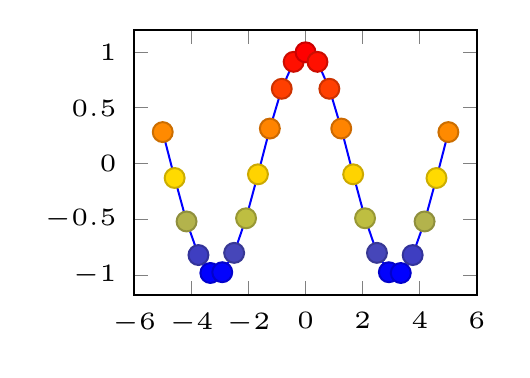
\begin{tikzpicture}[scale=1.8]
		\begin{axis}[tiny]
		\addplot+ [scatter] {cos(deg(x))};
		\end{axis}
		\end{tikzpicture}

		\captionof{figure}{A figure.}
		\label{fig:test1}
	\end{minipage}%
	\begin{minipage}{.48\textwidth}
		\centering
		
		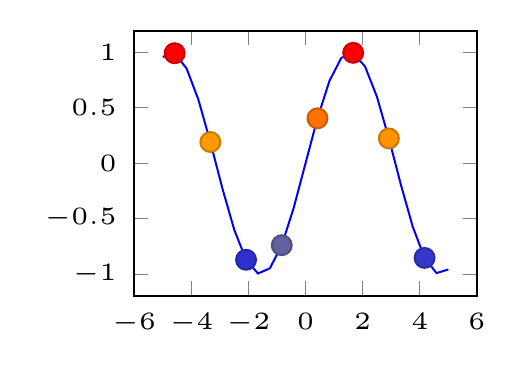
\begin{tikzpicture}[scale=1.8]
		\begin{axis}[tiny]
		\addplot+ [scatter,
		mark repeat=3,mark phase=2]
		{sin(deg(x))};
		\end{axis}
		\end{tikzpicture}
			
		\captionof{figure}{Another figure.}
		\label{fig:test2}
	\end{minipage}
\end{figure}


Fig. \ref{fig:test1} and Fig. \ref{fig:test2} represent two figures. In what follows, we draw an automaton using \LaTeX. All the sizes of elements in a drawing can be controlled.


\begin{figure}[htbp]
\begin{center}
	\begin{tikzpicture}
				[->,>=stealth',shorten >=1pt,auto,node distance=3.5cm,
				semithick,scale=.6,bend angle=45]
				%%%右箭头,箭头样式,自动适应,node默认间距,线条默认半粗,比例,默认弯角
				\tikzstyle{every state}=[fill=blue!30,draw=blue!75,text=black,minimum size=6mm,scale=1.5]
				%默认state样式为蓝色(0-100)填充,蓝色线条,黑色文本,最小size,比例
				%画出所有node
				\node[state,scale=0.4](0)                       {};
				%大括号内是node中的内容,(0)为该node的代号
				\node[state,scale=0.4](1) [below left of=0]     {};
				%[]内为(1)在(0)的左下位置,默认间距
				\node[state,scale=0.4](2) [below right of=0]    {};
				\node[draw=white]at(90:2)                       {}
				%一个不画出的node,由角坐标给出位置,注意这里还没有分号
				edge[<->](0);%其后可以直接定义edge,以分号结束指令
				
				
				%在node之间添加连线.第一个中括号中内容是连线的性质(颜色、弯曲方向和角度)
				%第二个括号中的内容是每条连线所附带的字母与连线的相对位置。有right\left\below\above可选
				\path 
				(0)edge [red,bend angle=30,bend right]node[above]{$\alpha$}      (1) %0到1
				(1)edge [bend angle=30,bend right]    node[right]{$\beta$}       (0)  
				(1)edge                               node[below]{$\lambda$}     (2)
				(2)edge [red,bend angle=30,bend right]node[above]{$\mu$}         (0)
				;%完整指令后以分号结束
			\end{tikzpicture}
\end{center}
\caption{This is an automaton.}
    \label{fig:my_label}
\end{figure}



\begin{figure}[htbp]
\centering
\begin{tikzpicture}[>=stealth]
	\node (state0) [draw=blue,fill=blue!20,xshift=2cm] {$(\{0,2\},\{0,2\})$};
	\node (state1) [draw=blue,fill=blue!20,left=1cm of state0.center,yshift=-1.5cm] {$(\{2\},\{0,2\})$};
    \node (state2) [draw=blue,fill=blue!20,right=1cm of state0.center,yshift=-1.5cm] {$(\{1,3\},\{0,2\})$};
    \node (state3) [draw=blue,fill=blue!20,below=1.3cm of state1.center] {$(\{1,3\},\{1,3\})$};
    \node (state4) [draw=blue,fill=blue!20,below=1.3cm of state2.center] {$(\{2\},\{2\})$};
    \node (state5) [draw=blue,fill=blue!20,below=1.3cm of state3.center] {$(\{2\},\{1,3\})$};
    \node (state6) [draw=blue,fill=blue!20,below=1.3cm of state4.center] {$(\{1,3\},\{2\})$};
    \draw[->,line width=1pt]  (2,1) -- (state0.north);
    \draw [->,line width=1pt,dashed] (state0) to node [right] {\footnotesize$a_{i}$} (state2);
	\draw [->,line width=1pt,dashed] (state1) to node [above] {\footnotesize$a_{i}$} (state2);
    \draw [->,line width=1pt,dashed] (state2.south west) to [in=340,out=200] node [above] {\footnotesize$c_{i}$} (state1.south east);
    \draw [->,line width=1pt,dashed] (state3.south) to node [left] {\footnotesize$c_{i}$} (state5.north);
	\draw [->,line width=1pt,dashed] (state5.east) to [in=330,out=10] node [left] {\footnotesize$a_{i}$} (state3.south east);
    \draw [->,line width=1pt,dashed] (state4.south) to  node [left] {\footnotesize$a_{i}$} (state6.north);
    \draw [->,line width=1pt,dashed] (state6.east) to [in=330,out=30] node [left] {\footnotesize$c_{i}$} (state4.south east);
    \draw [->,line width=1pt] (state1) to node [left] {\footnotesize$a$} (state3);
    \draw [->,line width=1pt] (state3) to node [below] {\footnotesize$c$} (state4);
    \draw [->,line width=1pt] (state4.north west) to node [above] {\footnotesize$a$} (state3.north east);
    \draw [->,line width=1pt] (state0.west) to [in=180,out=150] node [left] {\footnotesize$a$} (state3.west);
\end{tikzpicture}
\caption{Indicator automaton and verifier of the NFA in Fig. \ref{fig:my_label}}\label{indicator-NFA}
\end{figure}

\section{An example of table}
The table title is at the top of the table.

\begin{table}[htbp]	
	\centering
	\caption{A table.}
	\begin{tabular}[l]{@{}lcccccc}		
		\toprule		
		Class$^{\rm a}$ & $\gamma_1$ & $\gamma_2$$^{\rm b}$& $\langle \gamma \rangle$& $G$ & $|{ f}|$ & $\theta _{c}$ \\		
		\midrule	
		BL Lacs &5 & 36 & 7 & $-4.0$ & $1.0\times 10^{-2}$ & 10$^\circ$ \\		
		FSRQs & 5 & 40 & 11 & $-2.3$ & $0.5\times 10^{-2}$ & 14$^\circ$ \\		
		\bottomrule		
	\end{tabular}
	\label{tab:t1}
\end{table}

\begin{table}[htbp]  
\caption{Another table.}  
\begin{center}  
\begin{tabu} to 0.8\textwidth{X[c]|X[3,b]|X[2,l]|X[c]|X[3,m]|X[1,c]}  
%0.8\textwidth   为设置表格宽度  
%X[c]      表示这一列居中,所占比例为1,相当于X[1,c]  
%X[3,c]   表示这一列居中,所占比例为3,这列的宽度是X[c]列的3倍  
\hline  
$i$  &$x_i$              &$n_i$      &$i$    &$x_i$               &$n_i$\\  
\hline  
1    &0.5$\sim$0.64       &1           &8    &1.48$\sim$1.62      &53\\  
2    &0.64$\sim$0.78      &2           &9    &1.62$\sim$1.76      &25\\  
3    &0.78$\sim$0.92      &9           &10   &1.76$\sim$1.90      &19\\  
4    &0.92$\sim$1.06      &26          &11   &1.90$\sim$2.04      &16\\  
5    &1.06$\sim$1.20      &37          &12   &2.04$\sim$2.18      &3\\  
6    &1.20$\sim$1.34      &53          &13   &2.18$\sim$2.38      &1\\  
7    &1.34$\sim$1.48      &56          &     &                    & \\  
\hline  
\end{tabu}  
\end{center}  
\end{table}
